\documentclass[pointlessnumbers, abstracton, headsepline, a4paper]{scrartcl}

\usepackage[T1]{fontenc}
\usepackage[utf8]{inputenc}
\usepackage{graphicx}
\usepackage{microtype}
\usepackage{textcomp}
\usepackage{ellipsis, fixltx2e, mparhack, booktabs, longtable}
\usepackage[automark]{scrpage2}
\usepackage{multicol}
\usepackage{microtype}
\usepackage{listings}
\usepackage[a4paper]{geometry}
\usepackage[polish]{babel}
\usepackage{subfigure}
\usepackage{tikz}
\usetikzlibrary{arrows,positioning}

\usepackage{courier}
\lstset{
         basicstyle=\footnotesize\ttfamily, % Standardschrift
         %numbers=left,               % Ort der Zeilennummern
         numberstyle=\tiny,          % Stil der Zeilennummern
         %stepnumber=2,               % Abstand zwischen den Zeilennummern
         numbersep=5pt,              % Abstand der Nummern zum Text
         tabsize=2,                  % Groesse von Tabs
         extendedchars=true,         %
         breaklines=true,            % Zeilen werden Umgebrochen
         keywordstyle=\color{red},
         stringstyle=\color{white}\ttfamily, % Farbe der String
         showspaces=false,           % Leerzeichen anzeigen ?
         showtabs=false,             % Tabs anzeigen ?
         showstringspaces=false      % Leerzeichen in Strings anzeigen ?        
}

% part of the hyperref bundle
\usepackage{ifpdf}

\geometry{verbose,tmargin=3.5cm,bmargin=3.5cm}
\setlength{\parskip}{\medskipamount}
\setlength{\parindent}{0pt}

\clearscrheadfoot
\ohead{\\\headmark}
\ihead{
\includegraphics[scale=0.2]{img/zut2.jpg}}
\ofoot[\pagemark]{\pagemark}

% if pdflatex is used
\ifpdf

%set fonts for nicer pdf view
\IfFileExists{lmodern.sty}{\usepackage{lmodern}}
  {\usepackage[scaled=0.92]{helvet}
    \usepackage{mathptmx}
    \usepackage{courier} }
\fi

% the pages of the TOC are numbered roman
% and a pdf-bookmark for the TOC is added
\pagenumbering{arabic}
\let\myTOC\tableofcontents
\renewcommand\tableofcontents{\myTOC\clearpage\pagenumbering{arabic}}

\begin{document}
\begin{titlepage}

\begin{center}

\includegraphics[scale=0.5]{logos/zut.jpg}
\par
\end{center}

\begin{center}
\textsf{\textbf{\LARGE Wydział Informatyki}}
\end{center}{\LARGE}

\vspace{1.5cm}

\begin{center}
\textsf{\Large Metody sztucznej inteligencji}
\end{center}

\begin{center}
\textsf{\textbf{\Large Laboratorium 05 IUz-22 Urbaniak}}
\end{center}

\begin{center}
\textsf{\large Sprawozdanie}
\end{center}

\vspace{3.5cm}

\begin{center}
\begin{tabular}{ll}
Autor: & Sergiusz Urbaniak\tabularnewline
Grupa: & IUz-22\tabularnewline
Data: & \today\tabularnewline
\end{tabular}
\end{center}

\end{titlepage}

\tableofcontents

\section{Uczenie \texttt{dane\_sin1a}}

W następujących rysunkach są widoczne wykresy jak i błędy danych uczących na pliku \texttt{dane\_sin1a}. Zostały ustawione następujące wartości \texttt{spread}:
\begin{itemize}
\item 0.01
\item 0.06
\item 0.08
\item 1
\end{itemize}

Według wykresów błędu wynika że optymalna wartość \texttt{spread} jest 0.06.

\begin{figure}[!h]
\centering
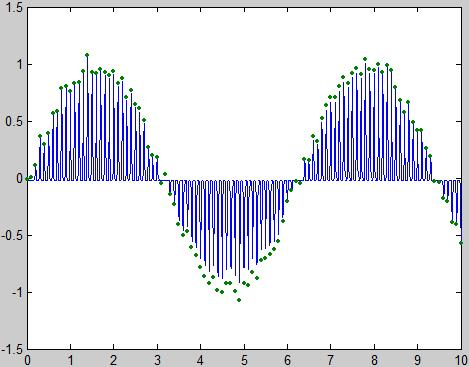
\includegraphics[scale=0.8]{src/0_01_wykres.png}\caption{\label{fig:0.01_wykres}Próbki (spread=0.01)}
\end{figure}

\begin{figure}[!h]
\centering
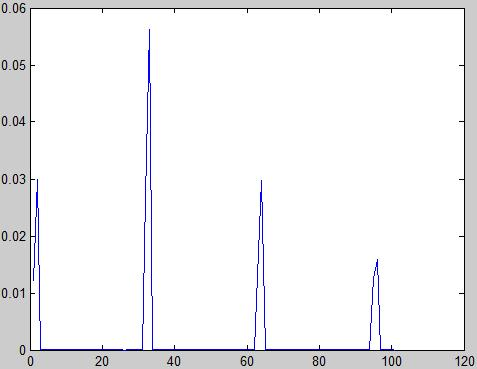
\includegraphics[scale=0.8]{src/0_01_blad.png}\caption{\label{fig:0.01_blad}Błąd (spread=0.01)}
\end{figure}

\begin{figure}[!h]
\centering
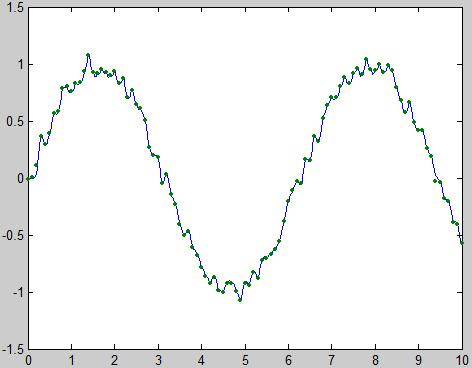
\includegraphics[scale=0.8]{src/0_06_wykres.png}\caption{\label{fig:0.06_wykres}Próbki (spread=0.06)}
\end{figure}

\begin{figure}[!h]
\centering
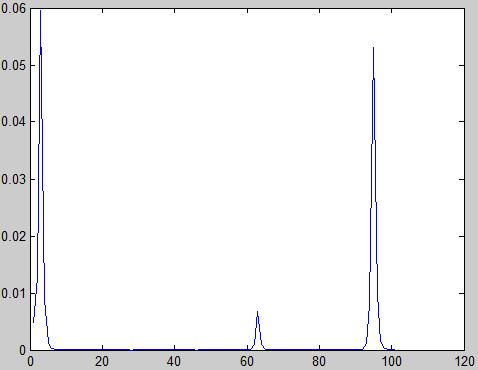
\includegraphics[scale=0.8]{src/0_06_blad.png}\caption{\label{fig:0.06_blad}Błąd (spread=0.06)}
\end{figure}

\begin{figure}[!h]
\centering
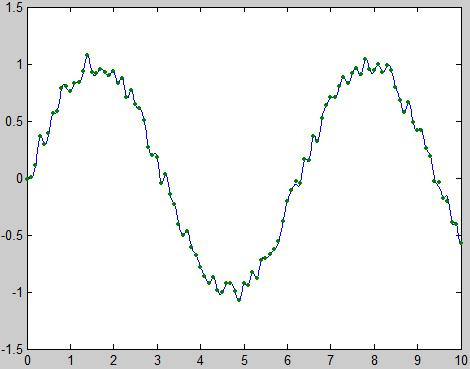
\includegraphics[scale=0.8]{src/0_08_wykres.png}\caption{\label{fig:0.08_wykres}Próbki (spread=0.08)}
\end{figure}

\begin{figure}[!h]
\centering
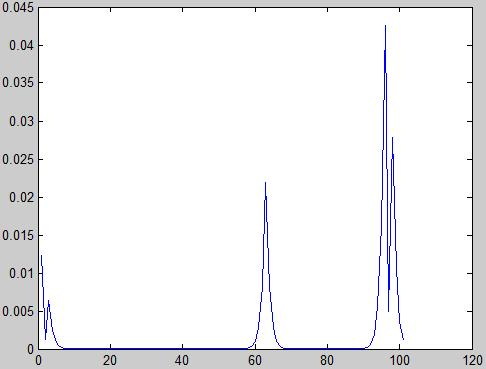
\includegraphics[scale=0.8]{src/0_08_blad.png}\caption{\label{fig:0.08_blad}Błąd (spread=0.08)}
\end{figure}

\begin{figure}[!h]
\centering
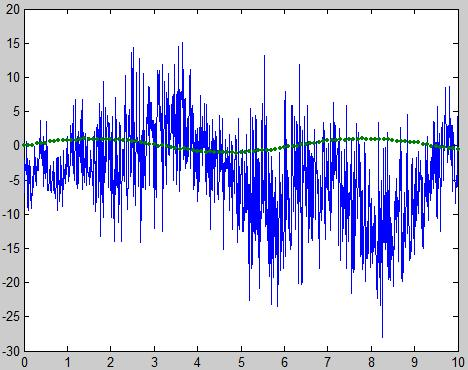
\includegraphics[scale=0.8]{src/1_wykres.png}\caption{\label{fig:0.08_wykres}Próbki (spread=1)}
\end{figure}

\begin{figure}[!h]
\centering
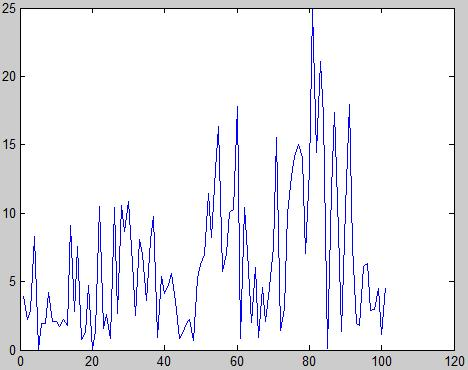
\includegraphics[scale=0.8]{src/1_blad.png}\caption{\label{fig:0.08_blad}Błąd (spread=1)}
\end{figure}



\end{document}
